%V105
\documentclass[
  bibliography=totoc,     % Literatur im Inhaltsverzeichnis
  captions=tableheading,  % Tabellenüberschriften
  titlepage=firstiscover, % Titelseite ist Deckblatt
]{scrartcl}

% Paket float verbessern
\usepackage{scrhack}

% Warnung, falls nochmal kompiliert werden muss
\usepackage[aux]{rerunfilecheck}

% unverzichtbare Mathe-Befehle
\usepackage{amsmath}
% viele Mathe-Symbole
\usepackage{amssymb}
% Erweiterungen für amsmath
\usepackage{mathtools}

% Fonteinstellungen
\usepackage{fontspec}
% Latin Modern Fonts werden automatisch geladen
% Alternativ zum Beispiel:
%\setromanfont{Libertinus Serif}
%\setsansfont{Libertinus Sans}
%\setmonofont{Libertinus Mono}

% Wenn man andere Schriftarten gesetzt hat,
% sollte man das Seiten-Layout neu berechnen lassen
\recalctypearea{}

% deutsche Spracheinstellungen
\usepackage{polyglossia}
\setmainlanguage{german}


\usepackage[
  math-style=ISO,    % ┐
  bold-style=ISO,    % │
  sans-style=italic, % │ ISO-Standard folgen
  nabla=upright,     % │
  partial=upright,   % ┘
  warnings-off={           % ┐
    mathtools-colon,       % │ unnötige Warnungen ausschalten
    mathtools-overbracket, % │
  },                       % ┘
]{unicode-math}

% traditionelle Fonts für Mathematik
\setmathfont{Latin Modern Math}
% Alternativ zum Beispiel:
%\setmathfont{Libertinus Math}

\setmathfont{XITS Math}[range={scr, bfscr}]
\setmathfont{XITS Math}[range={cal, bfcal}, StylisticSet=1]

% Zahlen und Einheiten
\usepackage[
  locale=DE,                   % deutsche Einstellungen
  separate-uncertainty=true,   % immer Fehler mit \pm
  per-mode=symbol-or-fraction, % / in inline math, fraction in display math
]{siunitx}

% chemische Formeln
\usepackage[
  version=4,
  math-greek=default, % ┐ mit unicode-math zusammenarbeiten
  text-greek=default, % ┘
]{mhchem}

% richtige Anführungszeichen
\usepackage[autostyle]{csquotes}

% schöne Brüche im Text
\usepackage{xfrac}

% Standardplatzierung für Floats einstellen
\usepackage{float}
\floatplacement{figure}{htbp}
\floatplacement{table}{htbp}

% Floats innerhalb einer Section halten
\usepackage[
  section, % Floats innerhalb der Section halten
  below,   % unterhalb der Section aber auf der selben Seite ist ok
]{placeins}

% Seite drehen für breite Tabellen: landscape Umgebung
\usepackage{pdflscape}

% Captions schöner machen.
\usepackage[
  labelfont=bf,        % Tabelle x: Abbildung y: ist jetzt fett
  font=small,          % Schrift etwas kleiner als Dokument
  width=0.9\textwidth, % maximale Breite einer Caption schmaler
]{caption}
% subfigure, subtable, subref
\usepackage{subcaption}

% Grafiken können eingebunden werden
\usepackage{graphicx}
% größere Variation von Dateinamen möglich
\usepackage{grffile}

% schöne Tabellen
\usepackage{booktabs}

% Verbesserungen am Schriftbild
\usepackage{microtype}

% Literaturverzeichnis
\usepackage[
  backend=biber,
]{biblatex}
% Quellendatenbank
\addbibresource{lit.bib}
\addbibresource{programme.bib}

% Hyperlinks im Dokument
\usepackage[
  unicode,        % Unicode in PDF-Attributen erlauben
  pdfusetitle,    % Titel, Autoren und Datum als PDF-Attribute
  pdfcreator={},  % ┐ PDF-Attribute säubern
  pdfproducer={}, % ┘
]{hyperref}
% erweiterte Bookmarks im PDF
\usepackage{bookmark}

% Trennung von Wörtern mit Strichen
\usepackage[shortcuts]{extdash}

\author{%
  Evelyn Romanjuk\\%
  \href{evelyn.romanjuk@tu-dortmund.de}{evelyn.romanjuk@tu-dortmund.de}%
  \texorpdfstring{\and}{,}%
  Ramona Kallo\\%
  \href{ramonagabriela.kallo@tu-dortmund.de}{ramonagabriela.kallo@tu-dortmund.de}%
}
\publishers{TU Dortmund – Fakultät Physik}

\begin{document}

\subject{V105 - Korrektur}
\title{Das magnetische Moment}
\author{
  Evelyn Romanjuk\\
  \href{mailto:evelyn.romanjuk@tu-dortmund.de}{evelyn.romanjuk@tu-dortmund.de}
  \texorpdfstring{\and}{,}
  Ramona Kallo\\
  \href{mailto:ramonagabriela.kallo@tu-dortmund.de}{ramonagabriela.kallo@tu-dortmund.de}}
\date{
  Durchführung: 10.11.17
  \hspace{3em}
  Abgabe der Korrektur: 01.12.17}
\publishers{TU Dortmund – Fakultät Physik}
\maketitle 
\newpage
\tableofcontents
\newpage

\section{Zielsetzung}
Im folgenden Versuch soll das Phänomen der Dispersion mithilfe einer Heliumlampe und eines Glasprismas untersucht werden. Genauer werden in zwei Versuchsteilen verschiedene Winkel bestimmt, aus denen auf das Dispersionsverhalten geschlossen werden kann.


\section{Theorie}
Tritt Licht mit der Lichtgeschwindigkeit $c$ in ein Medium ein, so wechselwirken die Lichtwellen mit den im Medium befindlichen Elektronen, wodurch sich die Geschwindigkeit des Lichtes  zu $v < c$ verringert. Beim Ein- oder Austreten des Lichts in oder aus 
dem Material unter einem Winkel ist ebenso zu beobachten, dass sich die Richtung des Lichtstrahls ändert, was Brechung genannt wird. Eine wichtige Größe, die dies charakterisiert, ist der Brechungsindex $n$, welcher sich aus dem Verhältnis der Lichtgeschwindigkeiten 
in den verschiedenen Medien ergibt:

\begin{equation}
n \:= \frac{v_1}{v_2} = \frac{c}{v}
\end{equation}

Der Brechungsindex kann außerdem auch über zwei Winkel bestimmt werden. Wichtig ist hierbei das Huygenssche Prinzip, das besagt, dass jeder Punkt einer Wellenfront das Zentrum einer neuen Elementarwelle ist. Fällt ein Lichtstrahl unter dem Winkel $\alpha$ gegen 
die Flächennormale auf ein Medium, so kommt es beim Eindringen zu einer Richtungsänderung. Innerhalb des Mediums breitet sich das Licht dann unter dem Winkel $\beta$ aus. 
In Abbildung \ref{fig:huygens} ist zu sehen, dass die Wellenfront zwischen den Punkten A und B im  Punkt A die Grenzfläche der beiden Medien bereits erreicht hat, während Punkt B die Grenzfläche erst nach $T = \frac{\overline{BC}}{v_1}$ erreicht. Nach diesem Zeitraum besitzt die Elemtenarwelle von 
Punkt A den Radius $Tv_2$, der Radius der Elementarwelle im Punkt C ist hingegen noch null. Ab diesem Zeitpunkt entsteht eine Wellenfront zwischen A‘ und C, wobei folgende Beziehungen gelten:

\begin{equation}
\begin{aligned}
\symup{sin}(\alpha) &= \frac{\overline{BC}}{\overline{AC}} = \frac{Tv_1}{\overline{AC}}, \\
\symup{sin}(\beta) &= \frac{\overline{A'A}}{\overline{AC}} = \frac{Tv_2}{\overline{AC}} \\
\end{aligned}
\end{equation}
Hieraus folgt:

\begin{equation}
\frac{\symup{sin}(\alpha)}{\symup{sin}(\beta)} = \frac{v_1}{v_2} = n.
\end{equation}

\begin{figure}[h!tbp]
	\centering
	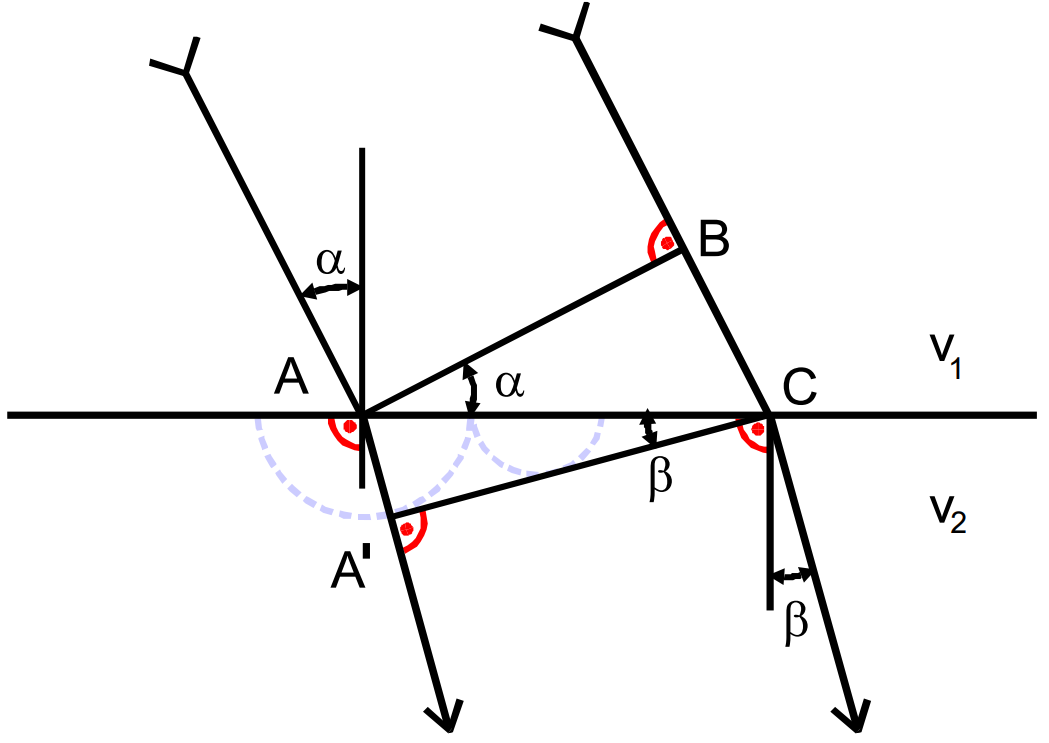
\includegraphics[width=0.6\linewidth]{hyugens.png}
	\caption{Skizze zum Huygenschen Prinzip.\cite[2]{anleitung402}}
	\label{fig:huygens}
\end{figure}


Weiterhin ist die Geschwindigkeit von Licht in einem Medium von der Frequenz abhängig und somit ist es auch der Brechungsindex $n$. Dieser Zusammenhang wird Dispersion genannt, wobei vor allem die Dispersionskurve der Form 

\begin{equation}
n = f(\lambda)
\end{equation}
wichtig ist. Diese kann mit einem Prisma  gewonnen werden, indem in diesem ein Lichtstrahl zweimal gebrochen wird. 

Zur Ableitung der Dispersionsgleichung werden Elektronen und Ionenrümpfe als Dipole betrachtet, die in dem elektrischen Wechselfeld der Lichtwellen zu schwingen beginnen. Dieses Modell ist nur für den sichtbaren Spektralbereich anwendbar, da die Absorption der Energie des Lichts hier zu vernachlässigen ist,
wohingegen bei Wellenlängen unterhalb des sichtbaren Bereichs Resonanzstellen auftreten, bei denen Absorption stattfindet.
Die einfallende Lichtwelle besitzt eine elektrische Feldstärke von

\begin{equation}
\vec{E} = \vec{E_0} e^{i\omega t}
\end{equation}
durch die eine periodische Kraft

\begin{equation}
\vec{F_{\text{e}}} = q_{\text{h}} \vec{E}
\end{equation}
auf die Ladungen $q_{\text{h}}$ ausgeübt wird, wodurch diese sich um $\vec{x_{\text{h}}}$ aus ihrer Gleichgewichtslage verschieben. Dadurch wirkt auf die Ladungen eine rücktreibende Kraft $\vec{F_{\text{r}}}$, die proportional zur Auslenkung ist, sowie auch eine Reibungskraft $\vec{F_{\text{d}}}$, welche
proportional zur Geschwindigkeit der Ladungsträger ist.
Hieraus ergibt sich für die Bewegung der Ladungsteilchen eine Differentialgleichung der Form:

\begin{equation}
m_{\text{h}} \frac{\symup{d}^2\vec{x_{\text{h}}}}{\symup{d}t^2} + f_{\text{h}}\frac{\symup{d}\vec{x_{\text{h}}}}{\symup{d}t} + a_{\text{h}}\vec{x_{\text{h}}} = q_{\text{h}} \vec{E_0} e^{i \omega t}
\end{equation}

Wird die Gleichung mit $\frac{N_{\text{h}} q_{\text{h}}}{m_{\text{h}}}$ erweitert, kann $\vec{x}_{\text{h}}$ durch die Polarisation $\vec{P}_{\text{h}}$ ersetzt werden:

\begin{equation}
\frac{\symup{d}^2\vec{P_{\text{h}}}}{\symup{d}t^2} + \frac{f_{\text{h}}}{m_{\text{h}}}\frac{\symup{d}\vec{P_{\text{h}}}}{\symup{d}t} + \frac{a_{\text{h}}}{m_{\text{h}}}\vec{P_{\text{h}}} = \frac{N_{\text{q}} q_{\text{h}}^2}{m_{\text{h}}} \vec{E_0} e^{i \omega t}.
\end{equation}

Mithilfe der Polarisation $\vec{P}$

\begin{equation}
\vec{P} = \sum_h \vec{P_{\text{h}}} = \sum_h N_{\text{h}} q_{\text{h}} \vec{x_{\text{h}}}
\end{equation}
und der Maxwellschen Relation $n^2 = \epsilon$  kann nun ein Zusammenhang zwischen Brechungsindex und Lichtfequenz gebildet werden:

\begin{equation}
\tilde{n}^2 = 1 + \sum_h \frac{1}{\omega_{\text{h}}^2 - \omega^2 + i \frac{f_{\text{h}}}{m_{\text{h}}} \omega} \frac{N_{\text{q}} q_{\text{h}}^2}{m_{\text{h}} \epsilon_0}
\end{equation}
Dies lässt sich in einen Real- und einen Imaginärteil aufspalten, woraus sich die Dispersionsgleichungen ergeben. Da die Frequenzen des sichtbaren Lichts relevant sind, wird nur der Bereich betrachtet, der sich weit von den Resonanzstellen entfernt befindet. Hierzu kann 

\begin{equation*}
n^2k \approx 0
\end{equation*}
angenommen werden. Wird nun $\omega$ durch die Wellenlänge $\lambda$ im Vakuum ersetzt, so ergibt sich

\begin{equation}
n^2(\lambda) = 1 + \sum_h \frac{N_{\text{h}} q_{\text{h}}^2}{4\pi^2 c^2 \epsilon_0 m_{\text{h}}} \frac{\lambda^2 \lambda_{\text{h}}^2}{\lambda^2 - \lambda_{\text{h}}^2}.
\label{eq:nquadrat}
\end{equation}
Nun können zwei Fallunterscheidungen vorgenommen werden.







\subsection{Fall: \texorpdfstring{$\lambda$}{Lambda} $>>$ \texorpdfstring{$\lambda_1$}{Lambda_1}}
In dem Fall, dass $\lambda$ viel größer ist als die Absorptionsstelle $\lambda_1$, kann \ref{eq:nquadrat} wie folgt entwickelt werden:

\begin{equation}
\begin{aligned}
n^2(\lambda) &= 1 + \frac{N_1 q_1^2 \lambda_1^2}{4 \pi^2 c^2 \epsilon_0 m_1} \biggl(1 + \biggl(\frac{\lambda_1}{\lambda}\biggr)^2 + \biggl(\frac{\lambda_1}{\lambda}\biggr)^4 + ... \biggr) \\
             &= A_0 + \frac{A_2}{\lambda^2} + \frac{A_4}{\lambda^4} + ...
\label{eq:fall1}
\end{aligned}
\end{equation}
mit $A_0$, $A_2$, $A_4 > 0$.




\subsection{Fall: \texorpdfstring{$\lambda$}{Lambda} $<<$ \texorpdfstring{$\lambda_1$}{Lambda_1}}
In dem Fall, dass $\lambda$ kleiner ist als die Absorptionsstelle $\lambda_1$, wird aus \ref{eq:nquadrat}:

\begin{equation}
\begin{aligned}
n^2(\lambda) &= 1 - \frac{N_1 q_1^2}{4 \pi^2 c^2 \epsilon_0 m_1} \biggl(\lambda^2 + \frac{\lambda^4}{\lambda_1^2} + \frac{\lambda^6}{\lambda_1^4} + ... \biggr) \\
             &= 1 - A'_2 \lambda^2 - A'_4 \lambda^4 - ...
\label{eq:fall2}
\end{aligned}
\end{equation}
mit $A'_{\text{i}} > 0$ für $i \geq 2$.

In Abbildung \ref{fig:dispersionskurven} sind die zugehörigen Kurvenverläufe zu sehen, welche sich durch ihre Krümmung unterscheiden. Genauer gilt bei \ref{eq:fall1}

\begin{equation}
\frac{\symup{d}^2 n^2 (\lambda)}{\symup{d} \lambda^2} > 0
\end{equation}

und im Fall \ref{eq:fall2}
\begin{equation}
\frac{\symup{d}^2n^2(\lambda)}{\symup{d}\lambda^2} < 0.
\end{equation}
Eine Gemeinsamkeit beider Fälle ist, dass es sich um normale Dispersion handelt, was bedeutet, dass der Brechungsindex bei zunehmender Wellenlänge abnimmt. Im Gegensatz dazu bedeutet die anormale Dispersion,
dass der Brechungsindex bei größer werdenen Wellenlängen ebenfalls zunimmt. Die anormale Dispersion ist in diesem Experiment allerdings nicht zu beobachten.

\begin{figure}[h!tbp]
	\centering
	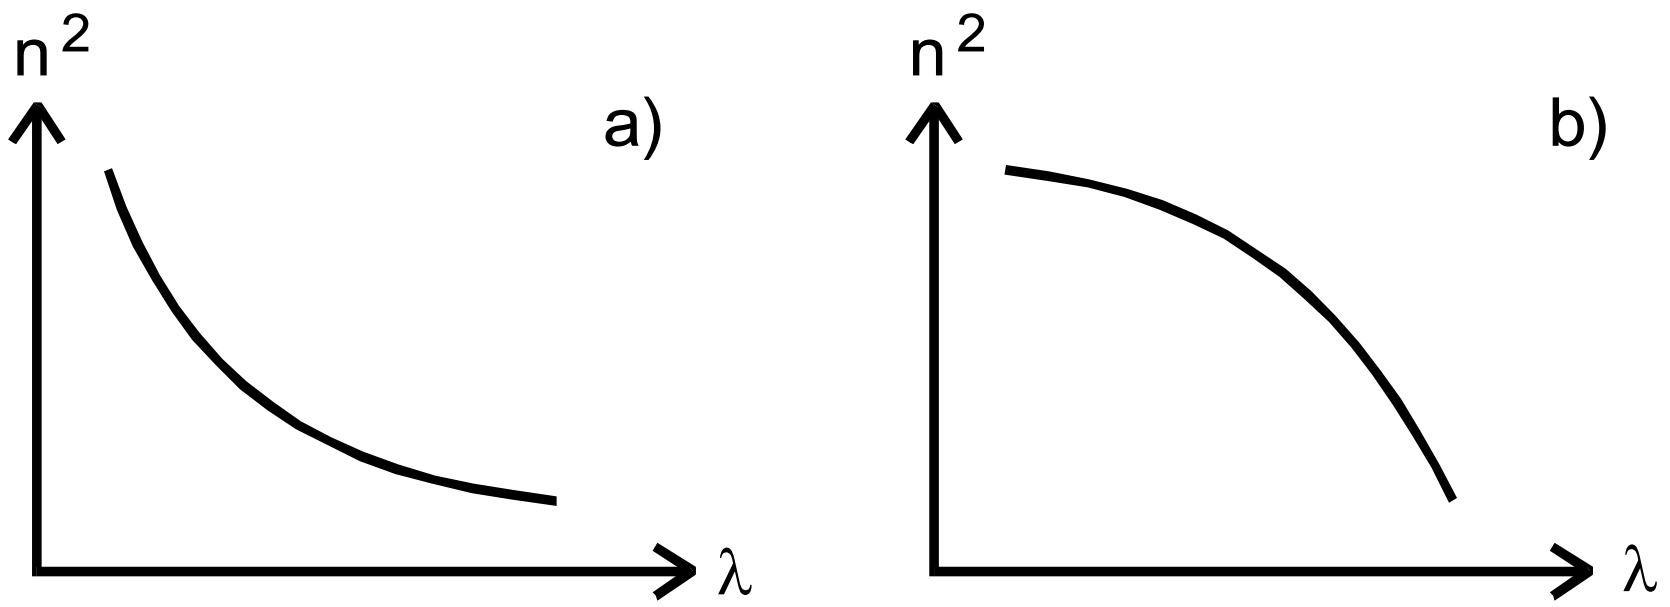
\includegraphics[width=0.7\linewidth]{dispersionskurven.png}
	\caption{Typische Dispersionskurven, a) nach \ref{eq:fall1}, b) nach \ref{eq:fall2}.\cite[7]{anleitung402}}
	\label{fig:dispersionskurven}
\end{figure}

\section{Aufbau und Durchführung}

Der generelle Aufbau des Geiger-Müller-Zählrohrs wurde bereits im vorherigen Kapitel erläutert. Wie in Abbildung \ref{fig:schaltbild} zu sehen ist, fließt die Ladung $Q$, die sich am Anodendraht sammelt, über den Widerstand $R$ und kann dann über einen 
Kondensator $C$ und einen Verstärker als Spannungsimpuls gemessen werden. Dieser kann auch über einen Oszillographen dargestellt werden.

\begin{figure}[h!tbp]
	\centering
	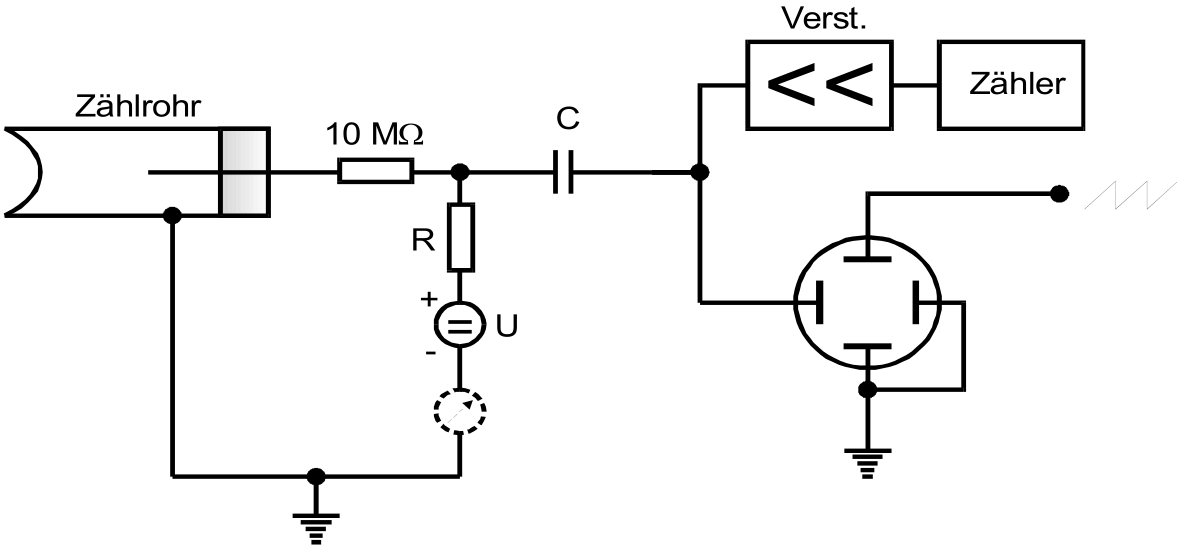
\includegraphics[width=0.8\linewidth]{../../schaltbild}
	\caption{Skizze der Messapparatur, \cite[7]{anleitung703}.}
	\label{fig:schaltbild}
\end{figure}

In diesem Versuch soll zunächst die Charakteristik des Zählrohrs aufgenommen werden. Dazu wird ein $\beta$-Strahler vor dem Zählrohr platziert. In 10\,V-Schritten werden für Spannungen zwischen 300 und 700\,V für jeweils 60\,s die Zählraten gemessen 
und gegeneinander aufgetragen.

Desweiteren können mithilfe des Oszilloskops die Nachentladungen, die für den Anstieg des Plateaus sorgen, dargestellt werden. Da es aus technischen Gründen nicht möglich ist, die Bilder auf dem Oszilloskop genauer zu analysieren, soll der Verlauf der
zu beobachtenden Kurve nur qualitativ erklärt werden.

Zudem soll die Totzeit auf zwei verschiedene Weisen gemessen werden. Die erste Messung erfolgt über das Oszilloskop. Dazu wird die Kurve so verschoben, dass mithilfe des Gitters und den Einstellungen am Oszilloskop die Totzeit abgelesen und die 
Erholungszeit grob abgeschätzt werden kann. Für die andere Methode wird eine zweite Strahlungsquelle eingesetzt, es handelt sich also um die sogenannte Zwei-Quellen-Methode. Die Grundlage hierfür ist wahre Impulsrate $N_{\text{w}}$ der eindringenden und absorbierten
Teilchen pro Zeiteinheit. Sie ist gegeben durch die registrierte Impulsrate $N_{\text{r}}$. $TN_{\text{r}}$ ist hierbei der Bruchteil der Messzeit, für die das Zählrohr unempfindlich ist:

\begin{equation*}
N_{\text{w}} = \frac{\text{Impulszahl}}{\text{Messzeit}} = \frac{N_{\text{r}} \cdot t}{(1-TN_{\text{r}})\cdot t} = \frac{N_{\text{r}}}{1-TN_{\text{r}}}
\label{eqn:impulsrate}
\end{equation*}
Im Experiment wird zunächst die Zählrate $N_1$ des ersten Präparats gemessen. Im Anschluss wird ein zweites Präparat hinzugefügt um die Zählrate $N_{1+2}$ beider Präparate zusammen zu messen, wobei darauf geachtet wird, dass das erste Präparat nicht bewegt wird.

Die Totzeit berechnet sich nach:
\begin{equation}
\label{eq:totzeit}
T \approx \frac{N_1 + N_2 - N_{1+2}}{2N_1 N_2}
\end{equation}


Im letzten Teil des Versuchs wird die pro Teilchen am Zählrohr freigesetzte Ladungsmenge untersucht. Es wird der Zählrohrstrom gemessen, welcher die transportierte Ladungsmenge $\Delta Q$ pro Zeitintervall $\Delta t$ repräsentiert, während der $Z$ Teilchen registriert werden:

\begin{equation}
\label{eq:ladung}
\bar{I} = \frac{\Delta Q}{\Delta t}\cdot Z.
\end{equation}
Dabei soll die Ladung $\Delta Q$ in Abhängigkeit von der Spannung $U$ gemessen werden.
\section{Auswertung}
\subsection{Fehlerrechnung}
In der folgenden Auswertung werden Mittelwerte mit
\begin{equation}
\bar{x} = \frac{1}{N} \sum_{\mathclap{i=1}}^N x_{\text{i}}
\label{eqn:mittelwert}
\end{equation}
und der zugehörige Fehler mit 
\begin{equation}
\Delta\bar{x} = \frac{1}{\sqrt{N}} \sqrt{\frac{1}{N-1}\sum_{\mathclap{i=1}}^N (x_{\text{i}}-\bar{x})^2}
\label{eqn:mittelwertfehler}
\end{equation}
berechnet. 
Beim Rechnen mit mehreren fehlerbehafteten Werten wird die Gauß'sche Fehlerfortpflanzung zur Berechnung des neuen Fehlers genutzt:
\begin{equation}
\Delta{f} = \sqrt{\sum_{i=1}^{N} \biggl(\frac{\delta{f}}{\delta{x}_{\text{i}}}\biggr)^2 \cdot (\Delta{x_{\text{i}}})^2}.
\label{eqn:gauss}
\end{equation}
\subsection{Bestimmung der Apparatekonstanten}
Um später die Viskosität von Wasser bei verschiedenen Temperaturen berechnen zu können, muss die Apparatekonstante $K_{\text{gr}}$ der großen Kugel bestimmt werden.
Hierfür werden zunächst die Dichten der beiden Kugeln aus den gegebenen Massen
\begin{equation*}
\begin{aligned}
m_{\text{kl}} &= 4.48 \cdot10^{-3} \symup{kg} \\
m_{\text{gr}} &= 4.97 \cdot 10^{-3}\symup{kg}
\end{aligned}
\end{equation*}
sowie den Radien der Kugeln aus Tabelle \eqref{tab:radienkugel} berechnet.

\begin{table}[htbp]
\centering
\caption{Radien der Kugeln}
\label{tab:radienkugel}
\begin{tabular}{
S[table-format=1.5, table-auto-round] 
S[table-format=1.5, table-auto-round]
}
\toprule
{Kleine Kugel} & {Große Kugel}  \\
{$r_{\text{kl}}$/$10^{-3}$m} & {$r_{\text{gr}}$/$10^{-3}$m} \\
\midrule
7.7545 & 7.763 \\
7.7545 & 7.7625  \\
7.75425 & 7.76275  \\
7.75425 & 7.76275 \\
7.76375 & 7.76325  \\
\bottomrule
\end{tabular}
\end{table}
Der Mittelwert der Radien wird mit Gleichung \eqref{eqn:mittelwert} und der Fehler des Mittelwerts mit Gleichung \eqref{eqn:mittelwertfehler} zu

\begin{equation*}
\begin{aligned}
r_{\text{kl}} &= (7.75445 \pm 0.00009) \cdot 10^{-3}\symup{m} \\
r_{\text{gr}} &= (7.76285 \pm 0.00013) \cdot 10^{-3}\symup{m}
\end{aligned}
\end{equation*}
berechnet. Die Volumina der Kugeln mit zugehörigem Fehler können dann mit Gleichung \eqref{eqn:gauss} errechnet werden. Es ergibt sich:
\begin{equation*}
\begin{aligned}
V_{\text{kl}} &= (1.95318 \pm 0.00007) \cdot 10^{-6}\symup{m^3} \\
V_{\text{gr}} &= (1.95953 \pm 0.00009) \cdot 10^{-6}\symup{m^3}
\end{aligned}
\end{equation*}
Hieraus können nun die Dichten der beiden Kugeln berechnet werden. Wieder wird Gleichung \eqref{eqn:gauss} für die Berechnung des Fehlerwertes genutzt.
\begin{equation*}
\begin{aligned}
\rho_{\text{kl}} &= (2293.65 \pm 0.08) \symup{\frac{kg}{m^3}} \\
\rho_{\text{gr}} &= (2536.321 \pm 0.116) \symup{\frac{kg}{m^3}}
\end{aligned}
\end{equation*}
 
Weiterhin wird für die Berechnung der Apparatekonstanten die Viskosität $\eta_{\text{RT}}$ von Wasser bei Raumtemperatur bestimmt. Verwendet werden
\begin{equation*}
\begin{aligned}
K_{\text{kl}} &= 7.64 \cdot 10^{-8}  \symup{\frac{Pa \cdot m^3}{kg}} \\
\rho_{\text{fl}} &= 998.2 \symup{\frac{kg}{m^3}}
\end{aligned}
\end{equation*}
wobei $K_{\text{kl}}$ die bereits gegebene Apparatekonstante der kleinen Kugel ist und $\rho_{\text{fl}}$ die Dichte von Wasser bei Raumtemperatur \cite{waterdensity}.
Zudem entnimmt man die Fallzeit der kleinen Kugel von
\begin{equation*}
t_{\text{kl}} = (12.42 \pm 0.09) \symup{s} \\
\end{equation*}
aus Tabelle \eqref{tab:fallzeitenkugel}.

\begin{table}[htbp]
\centering
\caption{Fallzeiten der Kugeln durch Wasser bei Raumtemperatur}
\label{tab:fallzeitenkugel}
\begin{tabular}{
S[table-format=2.2, table-auto-round] 
S[table-format=2.2, table-auto-round]
}
\toprule
{Kleine Kugel} & {Große Kugel}  \\
{$t_{\text{kl}}$/s} & {$t_{\text{gr}}$/s} \\
\midrule
12.03 & 72.63 \\
12.06 & 72.34 \\
12.24 & 73.27 \\
12.37 & 73.26 \\
12.40 & 74.61 \\
12.95 & 72.85 \\
12.60 & 72.82 \\
12.63 & 73.56 \\
12.44 & 74.28 \\
12.47 & 74.66 \\
\bottomrule
\end{tabular}
\end{table}

Nun lässt sich die Viskosität $\eta_{\text{RT}}$ mit Gleichung [K, DCIHTE; ZEIT] bestimmen. Sie beträgt
\begin{equation*}
\eta_{\text{RT}} = (1.23 \pm 0.09) \cdot 10^{-3} \symup{Pa \cdot s} \\
\end{equation*}
wobei der Fehlerwert wiederum aus der Gauß'schen Fehlerfortpflanzung \eqref{eqn:gauss} stammt.

Zuletzt wird Gleichung[K; DICHTE; ZEIT] nach $K_{\text{gr}}$ umgestellt. Mit den zuvor errechneten Werten ergibt sich eine Apparatekonstante von
\begin{equation*}
K_{\text{gr}} = (6.43 \pm 0.08) \cdot 10^{-8} \symup{\frac{Pa \cdot m^3}{kg}} \\
\end{equation*}

\subsection{Bestimmung der Temperaturabhängigkeit der Viskosität}
Wie bei der Bestimmung der Apparatekonstanten $K_{\text{gr}}$ kann Gleichung [K; DICHTE; ZEIT] für die Berechnung der Viskositäten von Wasser bei unterschiedlichen Temperaturen verwendet werden.
Hierbei sind $K_{\text{gr}}$, $\rho_{\text{gr}}$ und $t_{\text{gr}}$ fehlerbehaftete Größen, weshalb die Gauß'sche Fehlerfortpflanzung mit Gleichung \eqref{eqn:gauss} durchgeführt werden muss. 
Für die Dichte $\rho_{\text{fl}}$ von Wasser bei verschiedenen Temperaturen werden Literaturdaten \cite{waterdensity} verwendet.

\begin{table}[htbp]
\centering
\caption{Messdaten zur Bestimmung der Temperaturabhängigkeit der Viskosität von Wasser}
\label{tab:some_data}
\begin{tabular}{
S[table-format=3.2] 
S[table-format=2.2,table-figures-uncertainty=1]
S[table-format=3.2]
S[table-format=1.2, table-figures-uncertainty=1]
}
\toprule
{Temperatur} & {Fallzeit} & {Dichte Wasser} & {Viskosität} \\
{T/K} & {$t_{\text{gr}}$/s} & {$\rho_{\text{fl}}$/$\symup{\frac{kg}{m^3}}$} & {$\eta $/$10^{-3} \symup{Pa \cdot s}$}\\
\midrule
303.15   & 61.76 \pm 1.07 & 995.64 & 6.12 \pm 0.13 \\
307.15   & 55.7 \pm 0.4   & 994.37 & 5.52 \pm 0.08 \\
310.15   & 52.6 \pm 0.2   & 993.32 & 5.22 \pm 0.06 \\
313.20   & 49.5 \pm 0.2   & 992.19 & 4.91 \pm 0.06 \\
317.15   & 47.6 \pm 0.4   & 990.63 & 4.73 \pm 0.07 \\
321.15   & 43.5 \pm 0.1   & 988.93 & 4.33 \pm 0.05 \\
325.65   & 40.7 \pm 0.2   & 986.89 & 4.05 \pm 0.02 \\
329.65   & 37.9 \pm 0.4   & 984.97 & 3.78 \pm 0.06 \\
333.15   & 36.5 \pm 0.3   & 983.20 & 3.64 \pm 0.05 \\
336.15   & 34.9 \pm 0.1   & 981.63 & 3.49 \pm 0.04 \\
\bottomrule
\end{tabular}
\end{table}
Im Folgenden wird der natürliche Logarithmus der Viskosität gegen den Kehrwert der Temperatur aufgetragen, wie in Abbildung \eqref{fig:bildandrade} zu sehen ist. 
\begin{figure}[!h]
\centering
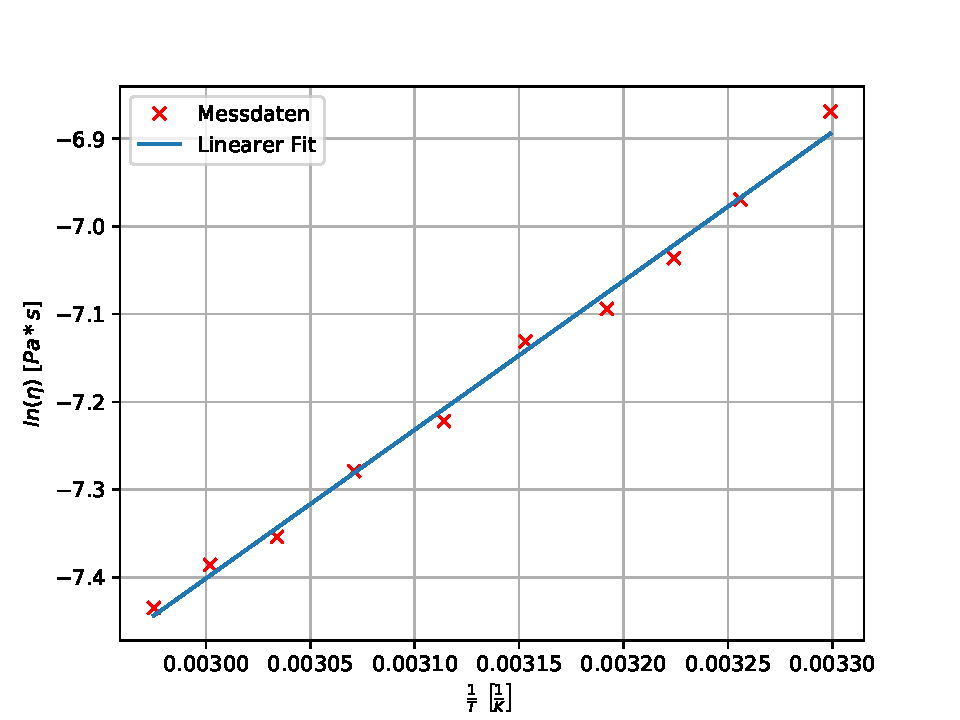
\includegraphics[scale=.9]{Andrade.pdf}
\caption{Bestimmung der Konstanten der Andradeschen Gleichung}
\label{fig:bildandrade}
\end{figure}

Mithilfe des Graphen lassen sich nun die Konstanten der 
Andradeschen Gleichung errechnen:
\begin{equation*}
\begin{aligned}
\eta(T) &= Ae^{\frac{B}{T}} \\
\iff ln(\eta) &= ln(A) + \frac{B}{T} \\
A &= (2.2 \pm 0.5)\cdot 10^{-5} \symup{Pa \cdot s} \\
B &= (1698.9 \pm 39.3) \symup{K} \\
\end{aligned}
\end{equation*}

\newpage
Zuletzt wird geprüft, ob die Strömung laminar oder turbulent ist. Hierzu wird die Reynoldszahl $Re_{\text{max}}$ der kleinen und der großen Kugel berechnet und dann mit dem kritischen Wert der 
Reynoldszahl $Re_{\text{krit}}$=1160 verglichen.
Wird in Gleichung [REYNOLDSZAHL] $d=2r_{\text{kl/gr}}$ und $v=\frac{x}{t_{\text{kl/gr}}}$ gesetzt, so ergibt sich
\begin{equation}
\begin{aligned}
Re = \frac{\rho \cdot 2r_{\text{kl/gr}} \cdot x}{\eta \cdot t_{\text{kl/gr}}}
\end{aligned}
\end{equation}
wobei x die Fallstrecke der Kugeln ist und $x=0.1\symup{m}$ \cite[3]{anleitung107} beträgt. Um den maximalen Wert der Reynoldszahl zu erhalten, wird jeweils die kleinste Fallzeit der Kugeln gewählt. Bei der 
großen Kugel entspricht dies der Fallzeit bei der höchsten Wassertemperatur.

Die Reynoldszahlen der beiden Kugel betragen damit
\begin{equation*}
\begin{aligned}
Re_{\text{max,kl}} &= 101.4 \pm 7.5 \\
Re_{\text{max,gr}} &= 12.5 \pm 0.2
\end{aligned}
\end{equation*}


\newpage 
\section{Diskussion}
Ziel dieses Versuches war es, das magnetische Moment eines Permanentmagneten auf drei verschiedene Weisen zu berechnen.
In jeder der Messmethoden gab es Fehlerquellen, die berücksichtigt werden müssen.
Zunächst die Gravitationsmethode. Hier könnten Fehler beim Vermessen der Billiardkugel mitsamt des Stiels auftreten sein. 
Zudem ist es möglich,dass die Abstände r von der Masse bis zur Kugel nur ungenau bestimmmt wurden und es ein Intervall gab, 
in der die Masse bei einem bestimmten Magnetfeld noch stabil war. Diese ungenauen Abstände würden sich damit direkt auf die
Berechnung von $\mu_{\text{Dipol}}$ auswirken. 

Bei der Methode über die Schwingungsdauer könnte es sein, dass die Auslenkungen nicht bei jeder Messung gleich groß waren und die 
Durchführungen somit nicht einheitlich, da Periodendauern dadurch vergrößert oder verkleinert wurden. Bei kleinen Periodendauern könnten
sich außerdem Fehler beim Stoppen der Zeit ergeben haben. 

Zuletzt gab es auch bei der Präzessionsmethode einige Fehlerquellen. Zunächst musste die Kugel in Rotation und in einen stabilen Zustand
versetzt werden. Wenn dies gelungen war, präzidierte die Kugel häufig schon, bevor der Strom richtig eingestellt wurde. Außerdem kam
es auch hier, wie in der Schwingungsmethode, vor, dass die Kugel nicht immer gleich stark ausgelenkt wurde. Weiterhin ergaben sich 
sicherlich auch Fehler beim Messen der Periodendauer, da es nicht immer genau ersichtlich war, wann eine Periode erreicht wurde. 

Ferner spielte bei allen Messmethoden eine Rolle wie lange der Strom eingeschaltet war, weil beim Erwärmen des Spulendrahtes dessen
Widerstand ansteigt. Daraus würde folgen, dass das Magnetfeld schwächer wird, was sich auf die gesamte Berechnung der magnetischen
Momente der verschiedenen Messmethoden auswirkt. 

Die Ergebnisse dieses Versuchs sind die folgenden magnetischen Momente:

\begin{equation*}
\begin{aligned}
\mu_{\text{Dipol, Grav}} &= (0.0953 \pm 0.0115) \symup{\frac{J}{T}} \\
\mu_{\text{Dipol, Schwing}} &= (0.1028 \pm 2.4674) \symup{\frac{J}{T}} \\
\mu_{\text{Dipol, Präz}} &= (0.0887 \pm 0.0054) \symup{\frac{J}{T}} 
\end{aligned}
\end{equation*}

Diese Werte weichen mindestens mit $6.93\%$ und maximal mit $15.9\%$ voneinander ab. Es ist zu erkennen, dass das magnetische Moment,
das über die Schwingungsmethode bestimmt wurde, den größten Fehlerwert aufweist. Dagegen hat die Präzessionsmethode den kleinsten.
Auffällig ist hierbei, dass die Präzessionsmethode eigentlich die meisten Fehlerquellen hat, aber dennoch die Methode ist, bei 
der das magnetische Moment den kleinsten Fehlerwert hat.


\nocite{*}
\printbibliography

\end{document}